%!TEX program = xelatex

% 完整编译: xelatex -> bibtex -> xelatex -> xelatex
\documentclass[lang=cn,11pt,a4paper]{elegantpaper}

% 这个模板有一点点的问题,其引用好像不太形

\title{Learning with Sparsity}
\author{Zhenwei Lin }
% \institute{\href{https://elegantlatex.org/}{Elegant\LaTeX{} 项目组}}

% \version{0.08}
\date{\zhtoday}

\theoremstyle{plain}
\newtheorem{thm}{Theorem}[section]
\newtheorem{lem}{Lemma}[section]
\newtheorem{prop}{Proposition}[section]
% \newtheorem*{cor}{Corollary}[section]

% \theoremstyle{definition}[section]
\newtheorem{defn}{Definition}[section]
\newtheorem{conj}{Conjecture}[section]
\newtheorem{exmp}{Example}[section]

\theoremstyle{remark}
\newtheorem*{rem}{Remark}



\usepackage{appendix}
\usepackage{varioref}
\renewcommand{\appendixtocname}{附录}
\renewcommand{\appendixpagename}{附录}
\begin{document}

\maketitle

\begin{abstract}
% 本文为 \href{https://github.com/ElegantLaTeX/ElegantPaper/}{ElegantPaper} 的说明文档。此模板基于 \LaTeX{} 的 article 类,专为工作论文写作而设计。设计这个模板的初衷是让作者不用关心工作论文的格式,专心写作,从而有更加舒心的写作体验。如果你有其他问题、建议或者报告 bug,可以在 \href{https://github.com/ElegantLaTeX/ElegantPaper/issues}{Github::ElegantPaper/issues} 留言。如果你想了解更多 Elegant\LaTeX{} 项目组设计的模板,请访问 \href{https://github.com/ElegantLaTeX/}{Github::ElegantLaTeX}。
本文主要为几种稀疏模型的介绍:
\keywords{Lasso; Ridege   }
\end{abstract}

% \section{Linear Regression}
% dataset is $\left\{ (x_i,y_i) \right\}_{i=1}^N $,and the model is 
% \begin{equation}
%   \begin{aligned}
%     y &= x^T\beta+\epsilon\\
%     &E(\epsilon) = 0\\
%     &Var(\epsilon) < \infty
%   \end{aligned}
% \end{equation}

% \section{Computational perspective}

% $$ \min_{\beta} \frac{1}{2}\sum_{i=1}^{N}(y_i-x_i^T\beta)^2 = \frac{1}{2}\left\| Y-X\beta \right\|^2  $$

% where \begin{equation}
%     Y = \left[\begin{array}{c}
%       y_1\\\vdots\\y_N
%     \end{array} \right]\in R^N,
%     x_{n\times p} = \left[\begin{array}{c}
%       x_1^T\\\vdots\\x_N^T
%     \end{array} \right]
% \end{equation}

% 为什么这里不把 $\beta_0$ 单独给出,因为该数据是被标准化过后的数据,可以看到标准化后的数据其 $\beta_0$为0.

% $$ \nabla {L(\beta)} = x^T(Y-X\beta) = 0 \Rightarrow (x^Tx)\beta  = x^TY$$

% \begin{enumerate}
%   \item if $X^TX$ is invertible ,we have $\hat{\beta} = (X^TX)^{-1}X^TY$
%   \item if $n<p$ means the size of sample is too small, we have rank($X^TX$) = rank($XX^T$) $\leq$ n
%   \item collinearity  
% \end{enumerate}

% To solve these problems, using \textbf{Tikhoov Regulation} $\hat{\beta_{\lambda}} = (X^TX+\lambda I)^{-1}X^TY$ where $X^TX$ is a semidefinite matrix,and I is a positive definitive matrix.

% \textbf{Tikhoov Regulation} in model means Ridge Regression.

% \begin{equation}\nonumber
%   \begin{aligned}
%     \min_{\beta} \quad \frac{1}{2}\left\| Y-x\beta  \right\|^2+\lambda \left\| \beta \right\| ^2 \\
%     \Rightarrow \nabla{L(\beta)} = -X^T(Y-X\beta)+2\lambda \beta = 0\\
%     \Rightarrow \hat{\beta_{\lambda}} = (X^TX+\lambda I)^{-1}X^TY
%   \end{aligned}
% \end{equation}


% \section{Bayesian Perspective}

% 下面从贝叶斯的角度来对其进行一定的解释。

% \begin{equation}\nonumber
%   \begin{aligned}
%     y_i &= x_i^T\beta+\epsilon_i \quad \epsilon_i \sim N(0,1)\\
%     \therefore f(y_i|x_i) &= \frac{1}{\sqrt{2\pi}}exp \left\{ -\frac{(y_i-x_i^T\beta)^2}{2} \right\} \\
%     \Rightarrow \max _{\beta}&\log\prod_{i=1}^N f(y_i|x_i) \iff \min _{\beta} \frac{1}{2}\left\| Y-x\beta \right\| ^2
%   \end{aligned}
% \end{equation}


% by $ P(A|B) = \frac{P(A,B)}{P(B)} = \frac{P(B|A)P(A)}{P(B)} $ 

% prior(先验信息)(对 $\beta$ 的理解 )
% \begin{equation}\nonumber
%   \begin{aligned}
%     f(\beta) &= \frac{\lambda^{\frac{p}{2}}}{\sqrt{2\pi}}exp \left\{ -\lambda \left\| \beta \right\|^2  \right\} \\
%     \because f(y_i|x_i) &= \frac{1}{\sqrt{2\pi}}exp \left\{ -\frac{(y_i-x_i^T\beta)^2}{2} \right\} \\
%     \therefore p(\beta|y,x) &= \frac{P(Y|\beta,x)P(\beta|x)P(x)}{P(Y|x)P(x)} = \frac{P(Y|\beta,x)P(\beta|x)}{P(Y|x)} \propto P(Y|\beta,x)P(\beta|x) = P(Y|\beta,x)P(\beta)\\
%     &\iff \max_{\beta} P(Y|x,\beta) P(\beta)  
%     \iff \min _{\beta} \frac{1}{2}  \left\| Y- X\beta \right\| ^2+\tilde{\lambda}\left\| \beta \right\|^2 \quad where \tilde{\lambda} = \frac{\lambda}{2}
%   \end{aligned}
% \end{equation}

% 因为x与 $\beta$ 无关,所以 $P(\beta|x) = P(\beta)$成立。





% \section{Lasso(least absolute shrinkage and selection operator)}

% \begin{equation}\nonumber
%   \begin{aligned}
%     \min_{\beta}\quad \frac{1}{2}\left\| Y-x\beta  \right\|^2 \\
%     s.t. \left\| \beta \right\| _1 \leq t
%   \end{aligned}
% \end{equation}

% and the intution could be shown in the following graph.

% \begin{center}
%   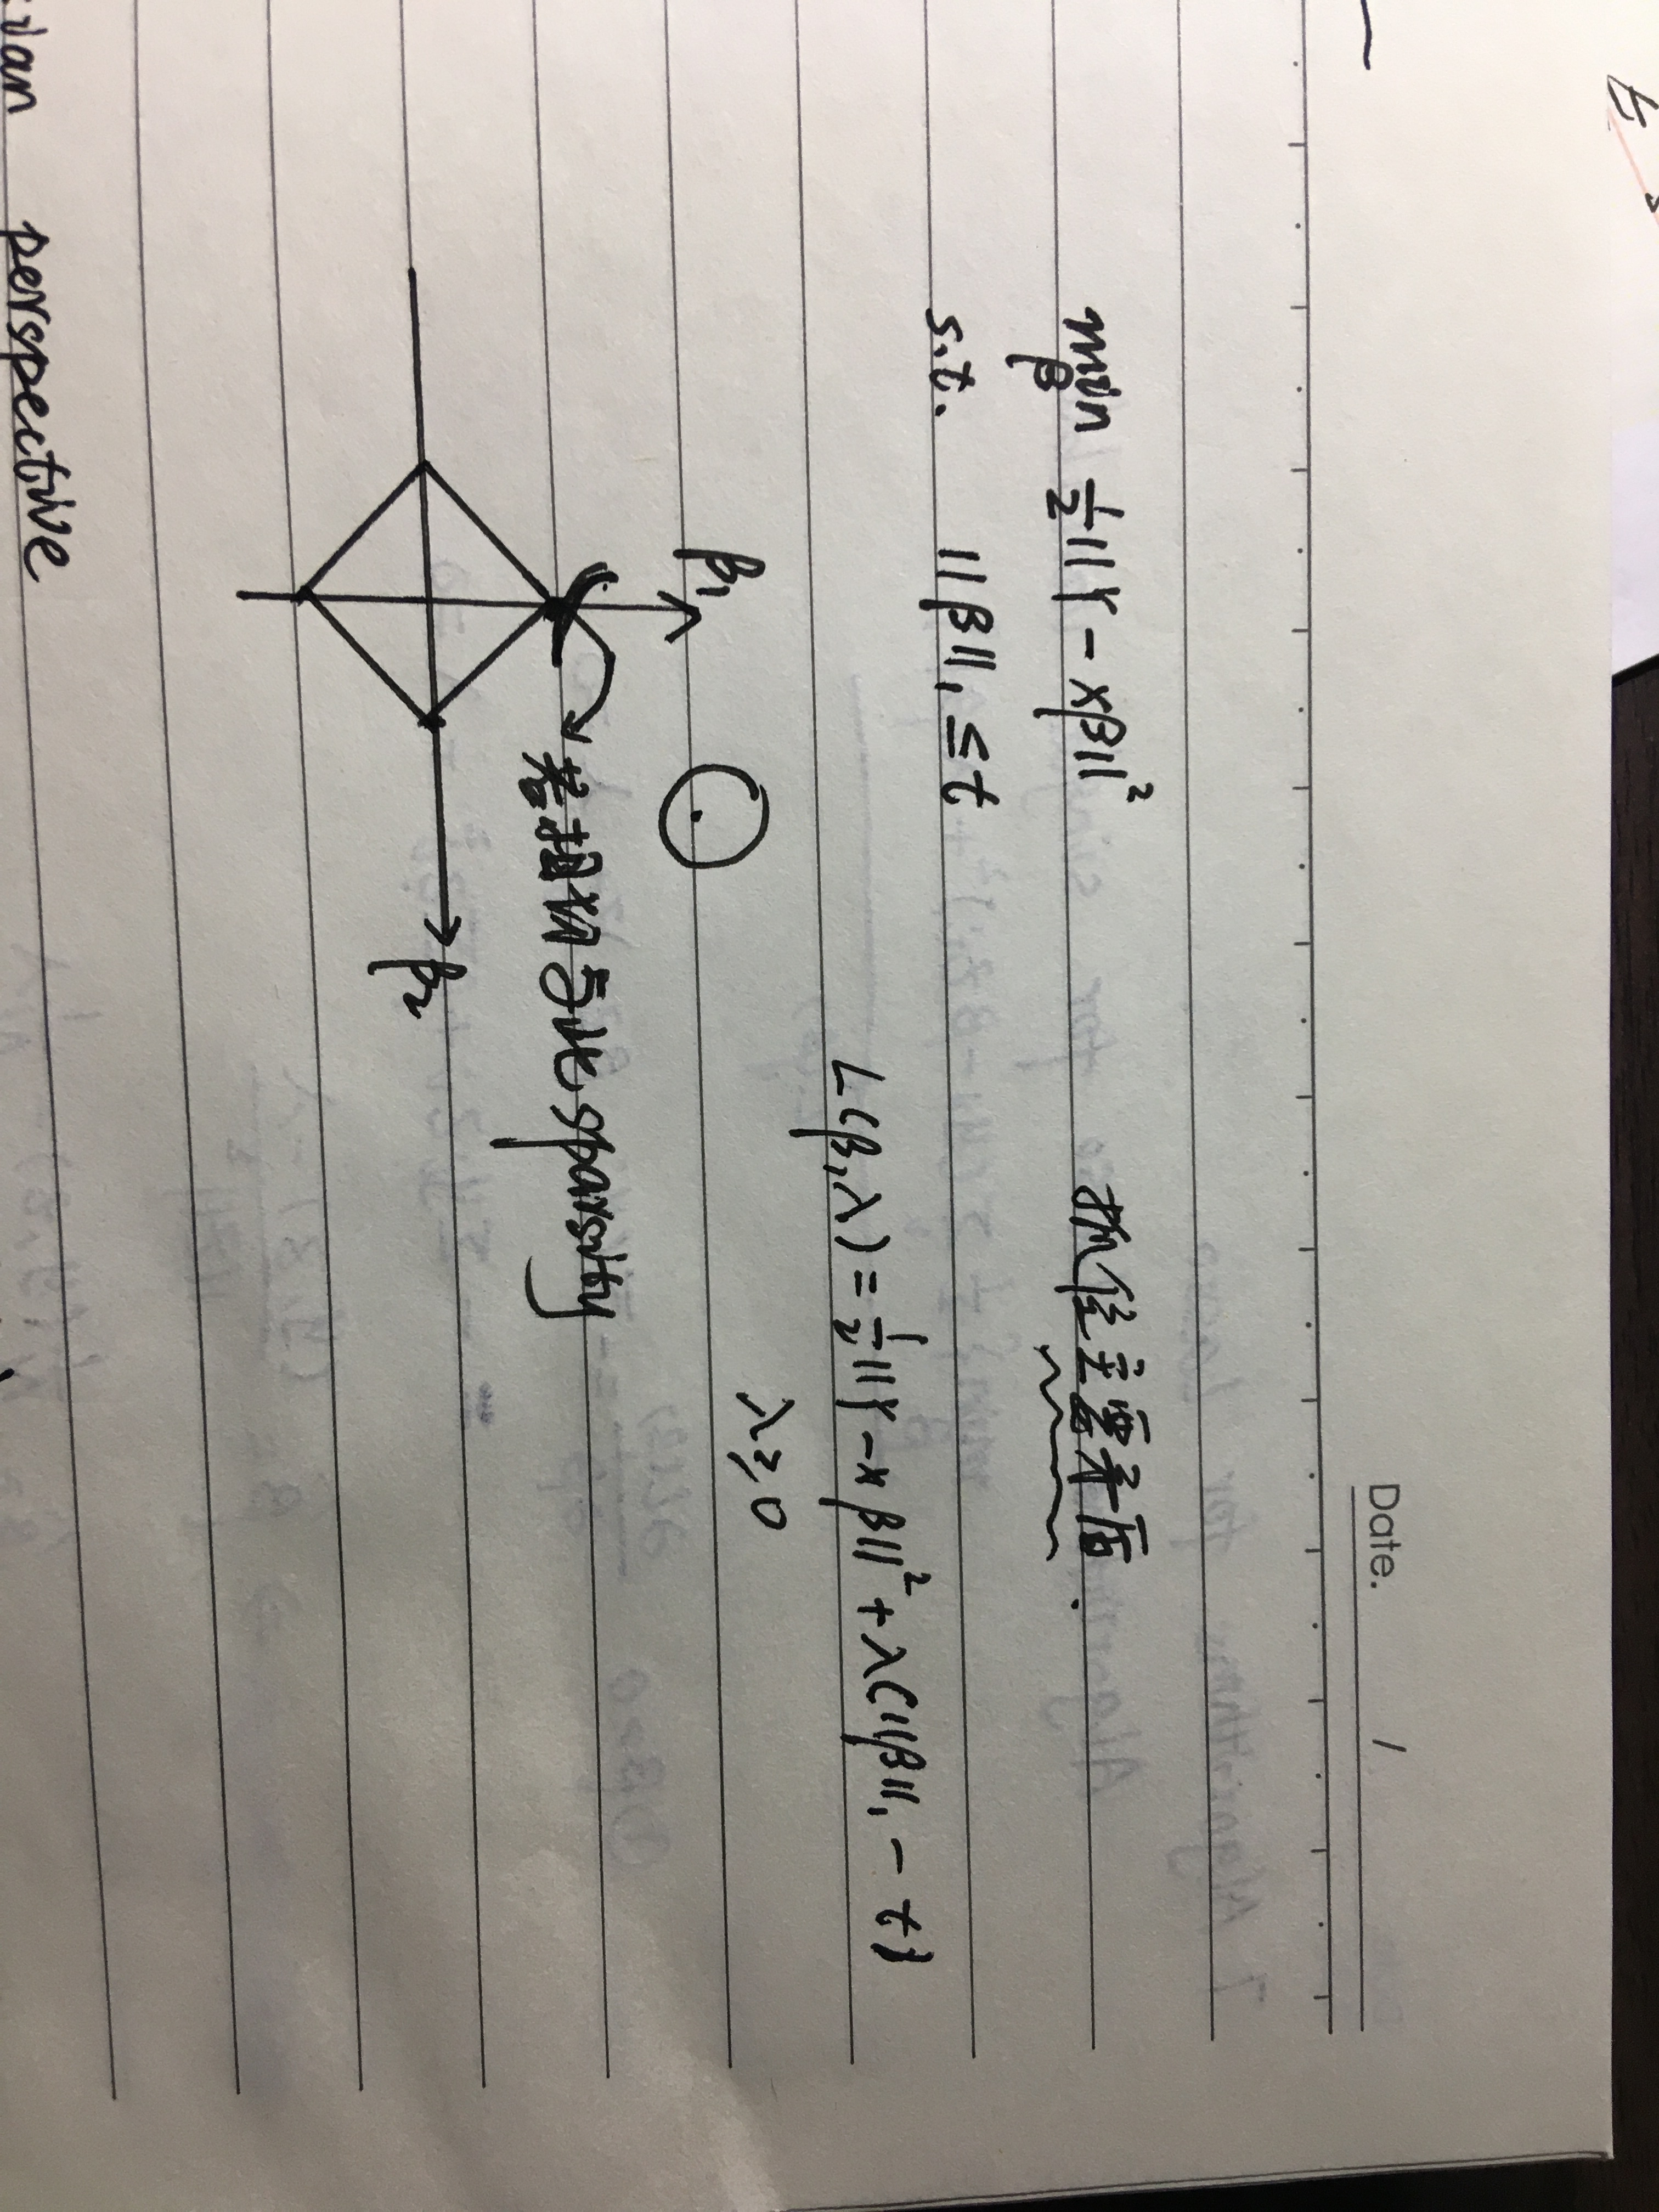
\includegraphics[width = 8cm,angle = 90]{fig/lasso.JPG}
% \end{center}

% In Bayesian Perspective:
% the prior is $P(B) = constant \times exp \left\{ -\lambda \left\| \beta \right\| _1 \right\}  $ (called laplace distribution)

% $$ p(B) \propto p(Y|x,\beta)p(\beta) $$
% $$ \max_{\beta} log \prod_{i=1}^N\exp \left\{ -\frac{(y_i-x_i^T\beta)^2}{2} \right\}\exp \left\{ -\lambda \left\| \beta \right\|_1 \right\} $$
% $$ \max_{\beta} -\frac{1}{2}\left\| Y-x\beta \right\|^2-\lambda \left\| \beta \right\| _1  $$
% $$ \min_{\beta} \frac{1}{2}\left\| Y-x\beta \right\|^2+\lambda \left\| \beta \right\| _1  (\lambda \geq 0)$$

% \section{Algorithms for lasso}

% \subsection{Algorithm 1(lasso for single variable)}

% \begin{equation}
%   \begin{array}{c}
%     \min_{\beta}\underbrace{\left\{ \frac{1}{2}\sum_{i} (y_i-\beta z_i)^2+\lambda \left\| \beta \right\|_1  \right\} }\\
%     L(\beta)    
%   \end{array}
% \end{equation}


% \begin{enumerate}
%   \item when $\beta >0$,\begin{equation}
%   \begin{aligned}
%     \frac{\partial{L(\beta)}}{\partial{\beta}} =& -\sum_i(y_i-\beta z_i)z_i+\lambda = 0\\
%     =&-\sum_i y_iz_i + \beta \sum_i z_i^2 + \lambda = 0\\
%     \Rightarrow & \hat{\beta} = \frac{(y,z)-\lambda}{ \left\| z \right\| ^2}\Rightarrow\hat{\beta} = \frac{\frac{1}{N}(y,z)-\frac{1}{N}\lambda}{ \frac{1}{N}\left\| z \right\| ^2}\\
%     \because&  \frac{1}{N}\left\| z \right\| ^2 = 1\\
%     \therefore &\hat{\beta} = \frac{1}{N}(y,z)-\frac{1}{N}\lambda = \frac{1}{N}(y,z)-\tilde{\lambda}
%   \end{aligned}
%   \end{equation}\nonumber
%   \item when $\beta$ < 0 ,similarly we have $$ \hat{\beta} = \frac{1}{N}(y,z)+\tilde{\lambda} $$
%   \item when $\beta = 0$ \begin{equation}\nonumber
% \begin{aligned}
%   0 &\in \partial{L(0)}\\
%   0 &\in -\frac{1}{N}\sum(y_i-\beta z_i)z_i + \lambda \partial \left| \beta \right| \\
%   \overset{\text{by} \beta = 0}{\iff} 0 &\in -\frac{1}{N}(y,z) + \lambda \partial \left| \beta \right| \\
%   \Rightarrow &\frac{1}{N}(y,z) = \lambda \partial \left| 0 \right| = [-\lambda,\lambda] 
% \end{aligned}
%   \end{equation} 
% \end{enumerate}

% summary: we have 
% \begin{equation}\nonumber
%   \begin{aligned}
%     \hat{\beta} = \left\{\begin{array}{ll}
%       \frac{1}{N}(y,z) - \tilde{\lambda} &\quad if \frac{1}{N} (y,z) > \tilde{\lambda}\\
%       0 &\quad if \left| \frac{1}{N} (y,z) \right| \leq \tilde{\lambda}\\
%       \frac{1}{N}(y,z) + \tilde{\lambda} &\quad if \frac{1}{N} (y,z) <- \tilde{\lambda}
%     \end{array}\right.
%   \end{aligned}
% \end{equation}

% 从计算结果来说,其内积即相关性越小,则其数值更偏向于0。

% so $\hat{\beta} = Soft_{\lambda}(\frac{1}{N}(y,z))$ 


% \subsection{Algorithm 2(Multivariable of orthogonal Design)}

% \begin{equation}\nonumber
%   \begin{aligned}
%     X_{n\times p }^T X &= I\\
%     \min_{\beta} \quad  \frac{1}{2N} \left\| Y-X\beta \right\|^2 &+ \lambda \left\| \beta \right\|_1 \\
%   \end{aligned}
% \end{equation}

% \begin{equation}\nonumber
%   \begin{aligned}
%     \left\| Y-x\beta \right\|^2 &= \left\| Y \right\| ^2 - 2(Y,X\beta)+\beta^TX^TX\beta\\
%     &= \left\| \beta \right\|^2 - 2(X^TY,\beta)+\left\| Y \right\| ^2\\
%     &= \left\| \beta - X^TY \right\| ^2+\left\| Y \right\|^2 - \left\| X^TY \right\| 
%   \end{aligned}
% \end{equation}

% $$ \iff min_{\beta} \left\{ \frac{1}{2N}\left\| \beta - x^{T}Y\right\|^2 + \lambda \left\| \beta \right\|_1 \right\}  $$
% can be decomposition.

% \subsection{Algorithm 3 (Cyclic Coordinate Descent)}

% \begin{equation}\nonumber
%   \beta \in \mathbf{R^p}  = (\beta_1,\cdots,\beta_p)^T
% \end{equation}

% and $\beta_2,\cdots,\beta_p$ is known.

% \begin{equation}
%   \begin{aligned}
%     \min_\beta& \left\{ \frac{1}{2N} \sum_{i=1}^N(y_i-\sum_{i=2}^p\beta_jx_j-\beta_1x_{i1})^2+\lambda \sum_{i=2}^p \left| \beta_i \right| + \lambda \left| \beta_1 \right|  \right\} \\
%     \min_{\beta}& \left\{ \frac{1}{2N} \sum_{i=1}^N(r_{i1}-\beta_1x_{i1})^2+\lambda \left| \beta_1 \right|  \right\} \\
%     \Rightarrow& \hat{\beta_1} = Soft_{\lambda}(\frac{1}{N}(r_i,x_1))
%   \end{aligned}
% \end{equation}
% 按照一个一个坐标轴分开进行优化。


% \subsection{ Algorithm 4 Proximal gradient descent}

% \begin{equation}\nonumber
%   \begin{aligned}
%     \begin{array}{c}
%       \min \left\{ \frac{1}{2N} \left\| Y-x\beta \right\|^2 
%     +\lambda \left\| \beta \right\| _1  \right\} 
%   \end{array}
%   \end{aligned}
% \end{equation}

% and we know $\frac{1}{2N} \left\| Y-x\beta \right\| ^2  $  is a $\beta$-smooth function.

% so \begin{equation}\nonumber
%   \begin{aligned}
%     &\left\| \nabla {f(\beta_1)} - \nabla {f(\beta_2)} \right\| \\
%     =&\left\| \frac{1}{N}X^T(Y-X\beta_1) - \frac{1}{N} X^T(Y-X\beta_2) \right\| \\
%     =&\frac{1}{N} \left\| X^TX(\beta_1-\beta_2) \right\| \leq \frac{\lambda_{max}(X^TX)}{N}\left\| \beta_1-\beta_2 \right\| \\
%     \Rightarrow b =& \frac{\lambda_{max}(X^TX)}{N}
%   \end{aligned}
% \end{equation}

% $$ \therefore \beta_{t+1} = prox_{g/b}(\beta_t - \frac{1}{b}\nabla{f(\beta)}) $$


% recall in definition, we have 
% $$ prox_{g/b}(z) = argmin_{x} \left\{ \frac{b}{2} \left\| x-z \right\| ^2+g(z) \right\}   $$


% $$ min_{x} \left\{ \frac{1}{2} \left\| x-z \right\| ^2+\frac{\lambda}{b} \left\| x \right\| _1 \right\} \Rightarrow prox_{g/b} = Soft_{\lambda/b}(z) $$

% \begin{equation}\nonumber
%   \begin{aligned}
%     \therefore \hat{\beta}_{t+1} =& Soft_{\lambda/b}(\beta_t+\frac{N}{\lambda_{max}(X^TX)}\frac{1}{N}X^T(Y-X\beta_t))\\
%     =&Soft_{\lambda/b} (\beta_t - \frac{X^TX}{\lambda_{\max}(X^TX)}\beta_t+\frac{X^TY}{\lambda_{max}(X^TX)})\\
%     =&Soft_{\lambda/b} \left\{ (I-\frac{X^TX}{\lambda_{max}(X^TX)})\beta_t+\frac{X^TY}{\lambda_{max}(X^TX)} \right\} 
%   \end{aligned}
% \end{equation}


% \subsection{Algorithm 5 : AGD $\rightarrow$ FISTA}

% \begin{equation}\nonumber
%   \begin{aligned}
%     \beta_0 =& 0,\alpha_1 = \beta_0,t=0\\
%     \beta_t = & Soft_{\lambda/b} \left\{ (I-\frac{X^TX}{\lambda _ {max}(X^TX)})\alpha_t+\frac{X^TY}{\lambda_{max}(X^TX)} \right\} \\
%     a_{t+1} =& \frac{1+\sqrt{1+4a_t^2}}{2}\\
%     \alpha_{t+1} =& \beta_t+\frac{a_t-1}{a_{t+1}}(\beta_t-\beta_{t+1})
%   \end{aligned}
% \end{equation}

% and the convergence speed is :$O(\frac{1}{T^2})$ 






% \subsection{Algorithm6:ADMM}

% \begin{equation}\nonumber
%   \begin{aligned}
%     \min_{\beta}\quad& \left\{ \frac{1}{2N} \left\| Y-X\beta \right\|^2+\lambda \left\| \beta \right\| _1  \right\} \\
%     \iff \min_{\beta} & \quad \left\{ \frac{1}{2N}  \left\| Y-X\beta \right\|^2 \right\} \\
%     s.t. &\quad \beta- \alpha = 0
%   \end{aligned}
% \end{equation}

% \begin{equation}\nonumber
%   \begin{aligned}
%     L(\beta,\alpha,v) =& \frac{1}{2N} \left\| Y-x\beta \right\|^2+\lambda \left\| \alpha \right\| _1 + v^T(\beta-\alpha) + \frac{\rho}{2} \left\| \beta-\alpha \right\|^2\\
%     \frac{\partial{L}}{\partial{\beta}} =& -\frac{1}{N} X^T(Y-X\beta)+v+\rho (\beta-\alpha)\\
%     =&(\frac{1}{N}X^TX + \rho I)\beta + v - \frac{1}{N}X^TY-\rho \alpha = 0\\
%     \Rightarrow \hat{\beta} =& (\frac{1}{N}X^TX+\rho I)^{-1}(\frac{1}{N}X^TY-v+\rho \alpha)
%   \end{aligned}
% \end{equation}

% for $\alpha$ :
% \begin{equation}\nonumber
%   \begin{aligned}
%     \min _{\alpha} &\left\{ \frac{\rho}{2} \left\| \alpha-\beta\right\|^2 - v^T(\alpha - \beta) +\lambda \left\| \alpha \right\| _1  \right\} \\
%     \iff  & \min _{\alpha} \left\{ \frac{\rho}{2} \left\| \alpha-\beta-\frac{v}{\rho}\right\|^2 +\lambda \left\| \alpha \right\| _1  \right\} \\
%     \iff & \min _{\alpha} \left\{ \frac{1}{2} \left\| \alpha-\beta-\frac{v}{\rho}\right\|^2 +\frac{\lambda}{\rho} \left\| \alpha \right\| _1  \right\} \\
%     \Rightarrow &\hat{\alpha} = Soft_{\lambda/\rho}(\beta+\frac{v}{\rho})\\
%     \therefore \beta_{t+1} &= (\frac{1}{N}X^TX+\rho I)^{-1}(\frac{1}{N}X^TY - v+\rho \alpha_t)\\
%     \alpha_{t+1} &= Soft_{\lambda/\rho}(\beta_{t+1} - \frac{v_t}{\rho})\\
% v_{t+1} &= v_t+\rho(\beta_{t+1} - \alpha_{t+1})
%   \end{aligned}
% \end{equation}

% \subsection{Alogrithm 7: Dual Method}
% \begin{equation}\nonumber
%   \begin{aligned}
%     \min_{\beta}&\quad \left\{ \frac{1}{2N} \left\| Y-X\beta \right\|^2+\lambda \left\| \beta \right\| _1  \right\} \\
%     \min_{\beta}&\quad \left\{ \sup_{\alpha} \left\{ (\alpha,Y-X\beta)-\frac{1}{2} \left\| \alpha \right\|^2  \right\} +\lambda \sup_{\lambda} \left\{ (\gamma,\beta) - \delta_{B_\infty}(\gamma) \right\}  \right\} 
%   \end{aligned}
% \end{equation}

% \section{Analysis of LASSO}

% 当我们使用数值方法求解出了 $\hat{\beta} = argmin \left\{ \frac{1}{2N} \left\| Y-X\beta \right\| ^2+\lambda \left\| \beta \right\| _1 \right\} $ 

% 但是我们考虑真实的模型为 $Y = X^T \beta^*+\epsilon$, where $\beta^*$ is real coefficient. 

% 这时我们对这个问题有三个方法可以来阐述其误差大小
% \begin{enumerate}[(a)]
%   {\setlength\itemindent{25pt} \item $l_2$ error $L_2(\hat{\beta},\beta^*) = \left\| \hat{\beta} - \beta^* \right\|_2 $ } 
%   {\setlength\itemindent{25pt} \item Prediction error : $L_p(\hat{\beta},\beta^*) = \frac{1}{N}\left\| X\beta^* - X\hat{\beta} \right\|^2 $} 
%   {\setlength\itemindent{25pt} \item Variable Selection Error : $\left\{ j|sign(\hat{\beta} ) \ne sign(\beta^*) \right\} $ } 
% \end{enumerate}

% 下面考虑第一种从 $l_2$-error的角度来看问题。

% denote $\hat{v} = \hat{\beta} - \beta^* $
% $$\Rightarrow L_2(\hat{\beta},\beta^*) = \left\| \hat{v} \right\| $$

% $$ \Rightarrow L_{p}(\hat{\beta},\beta^*) = \frac{1}{N}\left\| x\hat{v} \right\|^2_2  $$


% recall:
% $\alpha$-strong convex function 
% $$f(y) - f(x) - (\nabla {f(x)},y-x) \geq \frac{\alpha}{2}  \left\| y-x \right\| $$

% \textbf{这里假设 $f(\beta)$是一个 $\alpha$ -strong convex function}

% 再对 $f(\hat{\beta})$ 在 $\beta^*$ 处进行taylor展开,则有 

% \begin{equation}
%   f(\hat{\beta}) - f(\beta^*) - (\nabla {f(\beta^*),\hat{\beta}-\beta^*}) = \frac{1}{2N}\hat{v}^Tx^Tx\hat{v}\geq \frac{\gamma}{2} \left\| \hat{v} \right\| ^2
% \end{equation}

% %设置不同的缩进长度
% % \begin{enumerate}
% %   \item This item is not indented
% %   {\setlength\itemindent{25pt} \item This item is indented}
% %   \item This item is not indented
% %   {\setlength\itemindent{25pt} \item This item is indented}
% %   {\setlength\itemindent{25pt} \item This item is indented}
% %   \item This item is not indented
% %   \end{enumerate}


% 由于无法认为 $X^TX$满秩,故在某些区域上满足该条件进行思考,鉴于此,我们有restricted strong convex 成立。

% \begin{definition}
%   Restricted Strong convex 
%   \begin{equation}\nonumber
%     \begin{aligned}
%       f(y) - f(x) - (\nabla {f(x)},y-x) \geq \frac{\gamma}{2}\left\| y-x \right\| ^2\quad \forall x,y,y-x \in C
%     \end{aligned}
%   \end{equation}
% \end{definition}

% \begin{definition}
%   Restricted Eigenvalue Condition(REC)
%   \begin{equation}\nonumber
%     \frac{\hat{v}^Tx^Tx\hat{v}}{N} \geq \gamma \left\| \hat{v} \right\| ^2 \quad \hat{v} \in C
%   \end{equation}
% \end{definition}


% 现在我们先假设REC条件成立,考虑以下两个lasso 形式

% \begin{enumerate}
%   \item 
%   \begin{equation}
%     \begin{aligned}
%     \min \quad &\frac{1}{2} \left\| Y-X\beta \right\|^2 \\
%     s.t. \quad& \left\| \beta \right\|_1 \leq R 
%   \end{aligned}
%   \end{equation}
%   \item Lagrangian Lasso\begin{equation}
%     \min_{\beta} \left\{ \frac{1}{2N} \left\| Y-X\beta \right\|^2+\lambda_{N}\left\| \beta \right\|_1   \right\} 
%   \end{equation}
% \end{enumerate}

% 那么C是哪个集合呢?
% 我们先有如下符号定义:
% \begin{equation}\nonumber
%   \left\| \beta^* \right\|_0 = k 
% \end{equation}
% 说明其有k个位置不为0
% \begin{equation}\nonumber
%   \begin{aligned}
%     S \subseteq \left\{ 1,2,\cdots,p \right\} \\
%     v_s = \left\{ v|v_j = 0,j \notin s  \right\} \\
%     v_{s^c} = \left\{ v|v_j=0,j \in s \right\} 
%   \end{aligned}
% \end{equation}

% \begin{example}
%   \begin{equation}
%     \begin{aligned}
%       v &= (1,2,3)\\
%       s &= \left\{ 2 \right\} \\
%       \Rightarrow& v_s = \left\{ (0,2,0) \right\}\\
%       \Rightarrow& v_{s^c} = \left\{ (1,0,3) \right\} 
%     \end{aligned}
%   \end{equation}
% \end{example}

% 因此我们特定的取
% \begin{equation}\nonumber
%   s = \left\{ i|\beta^*_i \ne 0 \right\} \\
%   \Rightarrow \left\| \beta^* \right\| _1 = \left\| \beta^*_s \right\| _1
% \end{equation}


% \begin{lemma}
%   Assume \begin{equation}\nonumber
%     \begin{aligned}
%       \hat{\beta} \in& \quad \underset{\left\| \beta \right\| _1 \leq R}{argmin} \left\{  \frac{1}{2N} \left\| Y-X\beta \right\| ^2 \right\} \\
%       \hat{v} &= \hat{\beta} - \beta^*
%     \end{aligned}
%   \end{equation} 

%   then $ \left\| \hat{v}_{s^c} \right\|_1 \leq \left\| \hat{v}_s \right\| _1   $  where s = $  \left\{ j|\beta^* \ne 0 \right\}  $ 
% \end{lemma}

% \begin{proof}
%   假设其在边界上达到最优
% \begin{equation}\nonumber
%   \begin{aligned}
%     R &= \left\| \beta^* \right\|_1 \geq \left\| \hat{\beta} \right\| _1 = \left\| \hat{v}+\beta^* \right\| _1 = \left\| \hat{v}_s+\hat{v}_{s^c}+\beta^* \right\|_1 \\&=\begin{array}{cc}
%       \underbrace{\left\| \hat{v}_{s^c}  \right\|_1}\\\text{\tiny 取出($\hat{\beta} - \beta^*$)中$\beta^*=0$的部分}
%     \end{array} +\begin{array}{cc}
%       \underbrace{\left\| \beta^*+\hat{v}_s \right\|_1 }\\\text{ \tiny 取出($\hat{\beta} - \beta^*$)中$\beta^*\ne0$的部分}
%     \end{array}
%     \overset{\text{triangle inequality}}{\geq} \left\| \beta^* \right\| _1 - \left\| \hat{v}_s \right\| _1 + \left\| \hat{v}_{s^c}   \right\|_1 \\
%     \Rightarrow& \left\| \beta^* \right\| _1 \geq \left\| \beta^* \right\| _1 - \left\| \hat{v}_s \right\| _1 + \left\| \hat{v}_{s^c}   \right\|_1 
%   \end{aligned}
% \end{equation}
% \end{proof}


% \begin{defn}
%   \begin{equation}
%     C(S,1) = \left\{ v| \left\| v_{s^c} \right\| _1 \leq 1 \left\| v_s \right\| _1 \right\} 
%   \end{equation}
% \end{defn}

% \begin{lemma}
%   \begin{equation}
%     \begin{aligned}
%       p \geq q \geq 1,\quad x \in R^d\\
%       \left\| x \right\| _p \leq \left\| x \right\| _q \leq d^{\frac{1}{q} - \frac{1}{p}} \left\| x \right\| _p
%     \end{aligned}
%   \end{equation}
%   等价范数,范数可以被同样上下限控制住。
% \end{lemma}
% \begin{theorem}
%   \textbf{Consider Constrainted LASSO}.Assume REC over C(S,1) then 
%   \begin{enumerate}[(a)]
%     {\setlength\itemindent{25pt}\item $ \left\| \hat{\beta} - \beta^* \right\| \leq \frac{4\sqrt{k}}{\gamma} \left\| \frac{x^T\epsilon}{N} \right\|_{\infty}  $ }
%     \setlength\itemindent{25pt}\item if we futher assume that $\epsilon \overset{i.i.d}{\sim} N(0,\sigma^2)$ then for any $0<\delta<1$ we have 
%     $$ \left\| \hat{\beta}-\beta^*  \right\|  _2 \leq C(\delta) \frac{4\sigma}{\gamma} \sqrt{\frac{k log P}{N}} $$ 依概率 $1-\delta$ 成立,其中P为维数P.
%   \end{enumerate}
% \end{theorem}


% \begin{proof}[(a)proof:]
%   Basci inequality
%   \begin{equation}\nonumber
%     \begin{aligned}
%       \hat{v} &= \hat{\beta} - \beta^*\\
%       \frac{1}{2N}\left\| Y-X\beta \right\|^2 &\leq \frac{1}{2N} \left\| Y-X\beta^* \right\| ^2 \qquad Y=X\beta^*+\epsilon 
%     \end{aligned}
%   \end{equation}
%   basic inequality 成立的原因在于 $\hat{\beta}$ 是其最小化后的结果,而 $\beta^*$却只是其中符合模型的最优解
%   \begin{equation}\nonumber
%     \begin{aligned}
%       &\Rightarrow \left\| Y-X\beta^*+X\beta^*-X\hat{\beta} \right\|^2 \leq \left\| \epsilon \right\| ^2\\
%       &\left\| \epsilon+X(\beta^*-\hat{\beta}) \right\|^2 \leq \left\| \epsilon \right\| ^2\\
% &\Rightarrow \left\| X\hat{v} \right\| ^2 \leq 2(X^T\epsilon,\hat{v})\\
% &\Rightarrow \frac{1}{N} \left\| X\hat{v} \right\| ^2 
% \overset{\text{\tiny Cauchy-Schwarz inequality 对任意对偶范数成立}}{\leq} 2 \left\| \frac{X^T\epsilon}{N} \right\|_{\infty} \left\| \hat{v} \right\| _1 \\
% &\overset{\text{by REC}}{\rightarrow}\frac{1}{N}\left\| X\hat{v} \right\| ^2_2 \geq \gamma \left\| \hat{v} \right\| _2^2\\
% &\left\| \hat{v} \right\|_1 = \left\| \hat{v}_s+\hat{v}_{s^c} \right\|_1 \leq 2 \left\| \hat{v}_s \right\| _1 \leq 2\sqrt{k} \left\| \hat{v}_s\right\| _2 \leq 2\sqrt{k} \left\| \hat{v}\right\| _2\\
% \Rightarrow& \gamma \left\| \hat{v} \right\| _2^2 \leq 2 \left\| \frac{X^T\epsilon}{N} \right\|_{\infty} \left\| \hat{v} \right\|_1 \leq 4\sqrt{k} \left\| \frac{X^T\epsilon}{N} \right\|_{\infty} \left\| \hat{v} \right\|_2 \\
% \Rightarrow &\left\| \hat{v} \right\| _2 \leq \frac{4 \sqrt{k}}{\gamma} \left\| \frac{X^T\epsilon}{N} \right\|_{\infty}    
%     \end{aligned}
%   \end{equation}  
% \end{proof}


% \begin{proof}[(b)proof:]
%   \begin{equation}\nonumber
%     \begin{aligned}
% \epsilon_i \sim N(0,\sigma^2)\quad
% X = (x_1,\cdots,x_p)\quad
% X^T\epsilon = \left(\begin{array}{l}
%   x_1^T\epsilon\\
%   x_2^T\epsilon\\
%   \vdots \\
%   x_p^T \epsilon
% \end{array}\right)\\
% \frac{x_1^T\epsilon}{N} \sim N(0,\frac{\sigma^2  \left\| x_i \right\| ^2}{N^2})\overset{\frac{\left\| x_i \right\| ^2}{N} = 1}{=} N(0,\frac{\sigma^2}{N})\\
% p(\left| z \right| \geq t ) \overset{z\sim N(0,1)}{\leq} 2 exp(-\frac{t^2}{2\sigma^2})\\
% \Rightarrow p( \left| \frac{ x_i^T\epsilon}{N}  \right| \geq t) \leq 2exp(-\frac{Nt^2}{2\sigma^2})\\
% p( \left\|  \frac{x_i^T\epsilon}{N} \right\| _{\infty} \geq t) \leq \sum_{j=1}^P p(\frac{\left| x_i^T\epsilon \right| }{N}\geq t) = \begin{array}{c}
%   \underbrace{2 P exp(-\frac{Nt^2}{2\sigma^2})}\\
%   \delta
% \end{array}
%     \end{aligned}
%   \end{equation}
%   无穷范数表示其中的最大值
%   \begin{equation}\nonumber
%     \begin{aligned}
%       \Rightarrow log(\frac{\delta}{2p}) = -\frac{Nt^2}{2\sigma^2}\\
%       t = \sqrt{\frac{2\sigma^2}{N}log(\frac{p}{2\delta})} = c(\delta)\cdot\sigma\sqrt{\frac{log(p)}{N}}
%     \end{aligned}
%   \end{equation}
%   代入a的结论即可得证。
% \end{proof}

% 这个定理想表达的主要有:
% \begin{enumerate}
%   \item $\sigma$ 越大, $\left\| \hat{\beta}-\beta^* \right\| $越大不好估计
%   \item k越大,信息量越大,则不好找最优解
%   \item want $\frac{log P}{N} \rightarrow 0$,we have $O(logP)<O(N)$同时要求k小点,eg:N=100,则有 $\Rightarrow P = exp(10)$   
% \end{enumerate}


% \textbf{Consider Lagrangian LASSO}

% \begin{lemma}
%   If $\lambda_N \geq \frac{2 \left\| x^T\epsilon \right\|_{\infty} }{N}$ then
%   $$ \hat{v} \in C(S,3) = \left\{ v| \left\| v_{s^c} \right\|_1 \leq 3 \left\| v_s \right\|_1  \right\}  $$ 
% \end{lemma}

% \begin{proof}
%   By Basic inequality,we have
%   \begin{equation}\nonumber
%     \begin{aligned}
%       &\frac{1}{2N} \left\| Y-X\hat{\beta} \right\| ^2+\lambda_{N}\left\| \hat{\beta }\right\| _1 \leq \frac{1}{2N} \left\| Y-X\beta^* \right\|^2+\lambda_N \left\| \beta^* \right\|_1 \\
%       \Rightarrow& 0 \leq \frac{1}{N} \left\| X\hat{v} \right\|^2 \leq \frac{\left\| X^T\epsilon \right\|_{\infty} }{N} \left\| \hat{v} \right\|_1+\lambda_{N}(\left\| \beta^* \right\|_1  - \left\| \hat{\beta} \right\|_1 )\\
%       \Rightarrow& 0 \leq \frac{\lambda_N}{2} \left\| \hat{v} \right\|_1 +\lambda_N(\left\| \beta^* \right\|_1- \left\| \hat{\beta} \right\|_1  )  \\
%       &\left\| \hat{\beta} \right\|_1 = \left\| \hat{v}+\beta^* \right\|_1 = \left\| \hat{v_s}+\beta^*+\hat{v}_{s^c} \right\|_1 = \left\| \hat{v}_s+\beta^* \right\|_1+\left\| \hat{v}_{s^c} \right\|_1 \geq \left\| \beta^* \right\|_1- \left\| \hat{v}_s \right\|_1+\left\| \hat{v}_{s^c} \right\|_1\\
%       \Rightarrow& \left\| \hat{v}_s \right\|_1-\left\| \hat{v}_{s^c} \right\|_1 \geq \left\| \beta^* \right\|_1 - \left\| \hat{\beta} \right\|_1\\
%       \Rightarrow& \frac{1}{2} (\left\| \hat{v}_s \right\|_1+ \left\| \hat{v}_{s^c} \right\|_1  )+(\left\| \hat{v}_s \right\|_1-\left\| \hat{v}_{s^c} \right\|  )            \geq 0\\
%       \Rightarrow & \left\| \hat{v}_{s^c} \right\|_1 \leq 2 \left\| \hat{v}_s \right\|_1  
%     \end{aligned}
%   \end{equation}
% \end{proof}

% \begin{theorem}
%   let us consider the \textbf{Lagrangian LASSO} problem, and assume that x satifies REC over C(S,3), then for any $\lambda_N \geq  2 \left\| \frac{X^T\epsilon}{N} \right\|_{\infty}$,we have 
%   \begin{enumerate}[(a)]
%     \item $\left\| \hat{\beta} - \beta^* \right\| _1 \leq \frac{3\sqrt{k}}{\gamma} \lambda_N$
%     \item If we futher assume $\epsilon \overset{i.i.d}{\sim} N(0,\sigma^2)$ ,then we have $\left\| \hat{\beta}-\beta^* \right\| \leq \frac{C(s)}{\gamma} \sigma \sqrt{\frac{k log P}{N}}$
%   \end{enumerate}
% \end{theorem}


% 你可以在谷歌学术,Mendeley,Endnote 中获得文献条目(bib item),然后把它们添加到 \lstinline{wpref.bib} 中。在文中引用的时候,引用它们的键值(bib key)即可。注意需要在编译的过程中添加 \hologo{BibTeX} 编译。

% 本模板还添加了 \lstinline{cite=numbers} 、\lstinline{cite=super} 和 \lstinline{cite=authoryear}  三个参考文献选项,用于设置参考文献格式的设置,默认为 \lstinline{numbers}。理工科类一般使用数字形式 \lstinline{numbers} 或者上标形式 \lstinline{super},而文科类多使用作者-年份 \lstinline{authoryear} 比较多。如果需要改为 \lstinline{cite=numbers}  或者  \lstinline{authoryear} ,可以使用
% \begin{lstlisting}
% \documentclass[cite=super]{elegantpaper} % super style ref style
% \documentclass[super]{elegantpaper}

% \documentclass[cite=authoryear]{elegantpaper} % author-year ref style
% \documentclass[authoryear]{elegantpaper}
% \end{lstlisting}


% \section{协作人员招募}
% 招募 Elegant\LaTeX{} 的协作人员,没有工资。工作内容:翻译 Elegant\LaTeX{} 系列模板相关的文稿(中翻英),维护模板的 wiki(主要涉及 Markdown),如果有公众号文稿写作经历的话,也可以帮忙写微信稿。本公告长期有效。

% 目前 ElegantLaTeX 共有 4 名协作人员,分别是
% \begin{itemize}
%   \item 官方文档翻译: \href{https://github.com/peggy2006xzyz}{YPY};
%   \item Github 维基维护: \href{https://github.com/izinngo}{Ingo Zinngo}、\href{https://github.com/xiaohao890809}{追寻原风景};
%   \item QQ 群管理员: \href{https://github.com/sikouhjw}{Sikouhjw}.
% \end{itemize}

% 在此感谢他们无私的奉献!


% \section{致谢}
% 截止到 2019 年 10 月 17 日,ElegantPaper v0.08 版本发布,ElegantPaper 模板在 Github 上的收藏数(star)达到了 164。在此特别感谢 China\TeX{} 以及 \href{http://www.latexstudio.net/}{\LaTeX{} 工作室}对于本系列模板的大力宣传与推广。

% 如果你喜欢我们的模板,你可以在 Github 上收藏(Star)我们的模板。
% \begin{figure}[htbp]
%   \centering
%   
\includegraphics[width=\textwidth]{star.png}
%   \caption{一键三连求赞}
% \end{figure}

% \section{捐赠}
% 如果您非常喜爱我们的模板,你还可以选择捐赠以表达您对我们模板和我的支持!

% \begin{figure}[htbp]
%   \centering
%   
\includegraphics[width=0.5\textwidth]{donate.jpg}
% \end{figure}

% \textbf{赞赏费用的使用解释权归 Elegant\LaTeX{} 所有,并且不接受监督,请自愿理性打赏}。10 元以上的赞赏,我们将列入捐赠榜,谢谢各位金主!

% \begin{table}[!htbp]
%   \centering
%   \caption{Elegant\LaTeX{} 系列模板捐赠榜}
%   \begin{tabular}{crcc}
%     \toprule
%     捐赠者   & 金额 & 时间 & 渠道 \\
%     \midrule
%     Lerh  & 10 元  & 2019/05/15 & 微信 \\
%     越过地平线 & 10 元    & 2019/05/15 & 微信 \\
%     大熊 &  20 元 & 2019/05/27 & 微信 \\
%     * 空 & 10 元 & 2019/05/30 & 微信\\
%     \href{http://www.latexstudio.net/}{latexstudio.net} & 666 元 & 2019/06/05 & 支付宝\\
%     Cassis & 11 元 & 2019/06/30 & 微信\\
%     * 君 & 10 元 & 2019/07/23 & 微信\\
%     * 萌 & 19 元 & 2019/08/28 & 微信 \\
%     曲豆豆 & 10 元 & 2019/08/28 & 微信 \\
%     李博 & 100 元 & 2019/10/06 & 微信\\
%     Njustsll & 10 元 & 2019/10/11 & 微信 \\
%   \bottomrule
%   \end{tabular}%
% \end{table}%

% \section{常见问题 FAQ}

% \begin{enumerate}[label=\arabic*).]
%   \item \textit{如何删除版本信息?}\\
%       导言区不写 \lstinline|\version{x.xx}| 即可。
%   \item \textit{如何删除日期?}\\
%       需要注意的是,与版本 \lstinline{\version} 不同的是,导言区不写或注释 \lstinline{\date} 的话,仍然会打印出当日日期,原因是 \lstinline{\date} 有默认参数。如果不需要日期的话,日期可以留空即可,也即 \lstinline|\date{}|。
%   \item \textit{如何获得中文日期?}\\
%       为了获得中文日期,必须在中文模式下\footnote{英文模式下,由于未加载中文宏包,无法输入中文。},使用 \lstinline|\date{\zhdate{2019/10/11}}|,如果需要当天的汉化日期,可以使用 \lstinline|\date{\zhtoday}|,这两个命令都来源于 \href{https://ctan.org/pkg/zhnumber}{\lstinline{zhnumber}} 宏包。
%   \item \textit{如何添加多个作者?}\\
%       在 \lstinline{\author} 里面使用 \lstinline{\and},作者单位可以用 \lstinline{\\} 换行。\begin{lstlisting}
% \author{author 1\\ org. 1 \and author 2 \\ org. 2 }
% \end{lstlisting}
%   \item \textit{如何添加中英文摘要?}\\
%       请参考 \href{https://github.com/ElegantLaTeX/ElegantPaper/issues/5}{Github::ElegantPaper/issues/5}
% \end{enumerate}

% \section{示例}

% 为了让大家更加清楚最终的论文效果,如下给出两篇使用 ElegantPaper 模板排版的工作论文示例,也欢迎大家“投稿”!

% \begin{enumerate}
%   \item \href{https://github.com/EthanDeng/bank-custody}{银行存管、投资者决策与 P2P 网络借贷规范发展};
%   \item \href{https://github.com/EthanDeng/risk-awareness}{互联网金融风险与投资者风险意识 —— 来自网贷平台交易数据的证据}。
% \end{enumerate}

% 这是一个最小示例文档(Minimal Example):
% \begin{lstlisting}
% \documentclass[lang=cn,a4paper,11pt]{elegantpaper}

% % title information
% \title{Working Paper Example}
% \author{Author Name} 
% \institute{Elegant\LaTeX{} Group}

% \version{1.00}
% \date{\today}

% \begin{document}

% \maketitle

% \begin{abstract}
% Your abstract goes here.
% \keywords{keyword1, keyword2}
% \end{abstract}

% \section{Introduction}
% The content of introduction section.

% \section{Conclusion}
% The content of conclusion section.

% \bibliography{wpref}

% \end{document}
% \end{lstlisting}

% \nocite{*}
% \bibliography{wpref}

% \appendix
% \appendixpage
% \addappheadtotoc
% \section{How I became inspired}

\end{document}
